\documentclass[12pt,a4paper]{article}
\usepackage[utf8]{inputenc}
\usepackage{a4wide}
\usepackage[czech]{babel}
\usepackage{amsmath}
\usepackage{amsfonts}
\usepackage{amssymb}
\usepackage{gensymb}
\usepackage{graphicx}
\usepackage[a4paper,top=20mm,bottom=20mm,left=20mm,right=20mm,nohead,dvips]{geometry}
\usepackage{listings}
\usepackage{hyperref}
\usepackage{url}

\usepackage{paralist}
\usepackage{amsthm}
\usepackage{url}
\usepackage{menukeys}
\usepackage{graphicx}
\usepackage{listings}
\usepackage{xcolor}
\usepackage{hhline}
\usepackage{siunitx}
\usepackage[most]{tcolorbox}
\usepackage{adjustbox}

%% Special colors definitions
\definecolor{background}{HTML}{F5DD9D}
\definecolor{symbolColorTop}{HTML}{FFECB3}
\definecolor{symbolColorBox}{HTML}{FFF9E5}
\definecolor{gray}{rgb}{0.25,0.25,0.25}
\definecolor{darkblue}{rgb}{0.0,0.0,0.6}
\definecolor{cyan}{rgb}{0.0,0.6,0.6}
\definecolor{lightblue}{rgb}{0.9,0.95,1.0}
\definecolor{darkgreen}{rgb}{0.0,0.6,0.0}
\definecolor{brown}{HTML}{A52A2A}
\definecolor{darkmagenta}{HTML}{8B008B}

\newcommand\Cpp{
\lstset{
	basicstyle=\ttfamily,
	columns=fullflexible,
	showstringspaces=false,
	tabsize=4,
	numbers=left,
	backgroundcolor = \color{lightblue},
	language=C++,
	identifierstyle=\color{brown},
	keywordstyle=\color{blue},
	stringstyle=\color{red},
	commentstyle=\color{darkgreen},
	morecomment=[l][\color{darkmagenta}]{\#}
}
}

\author{Bedřich Said}
\title{Specifikace SensorBoard v1.0}

\begin{document}
\maketitle

SensorBoard je autonomní elektronická deska se senzory, baterií a procesorem. Primárně je určena pro detekci a měření pohybu v prostoru. Ve verzi 1.0 jde o testovací prototyp, který obsahuje některé senzory a součástky navíc za účelem testování.

\quad\\

\begin{figure}[h!]
  \centering
  \begin{minipage}{10cm}
    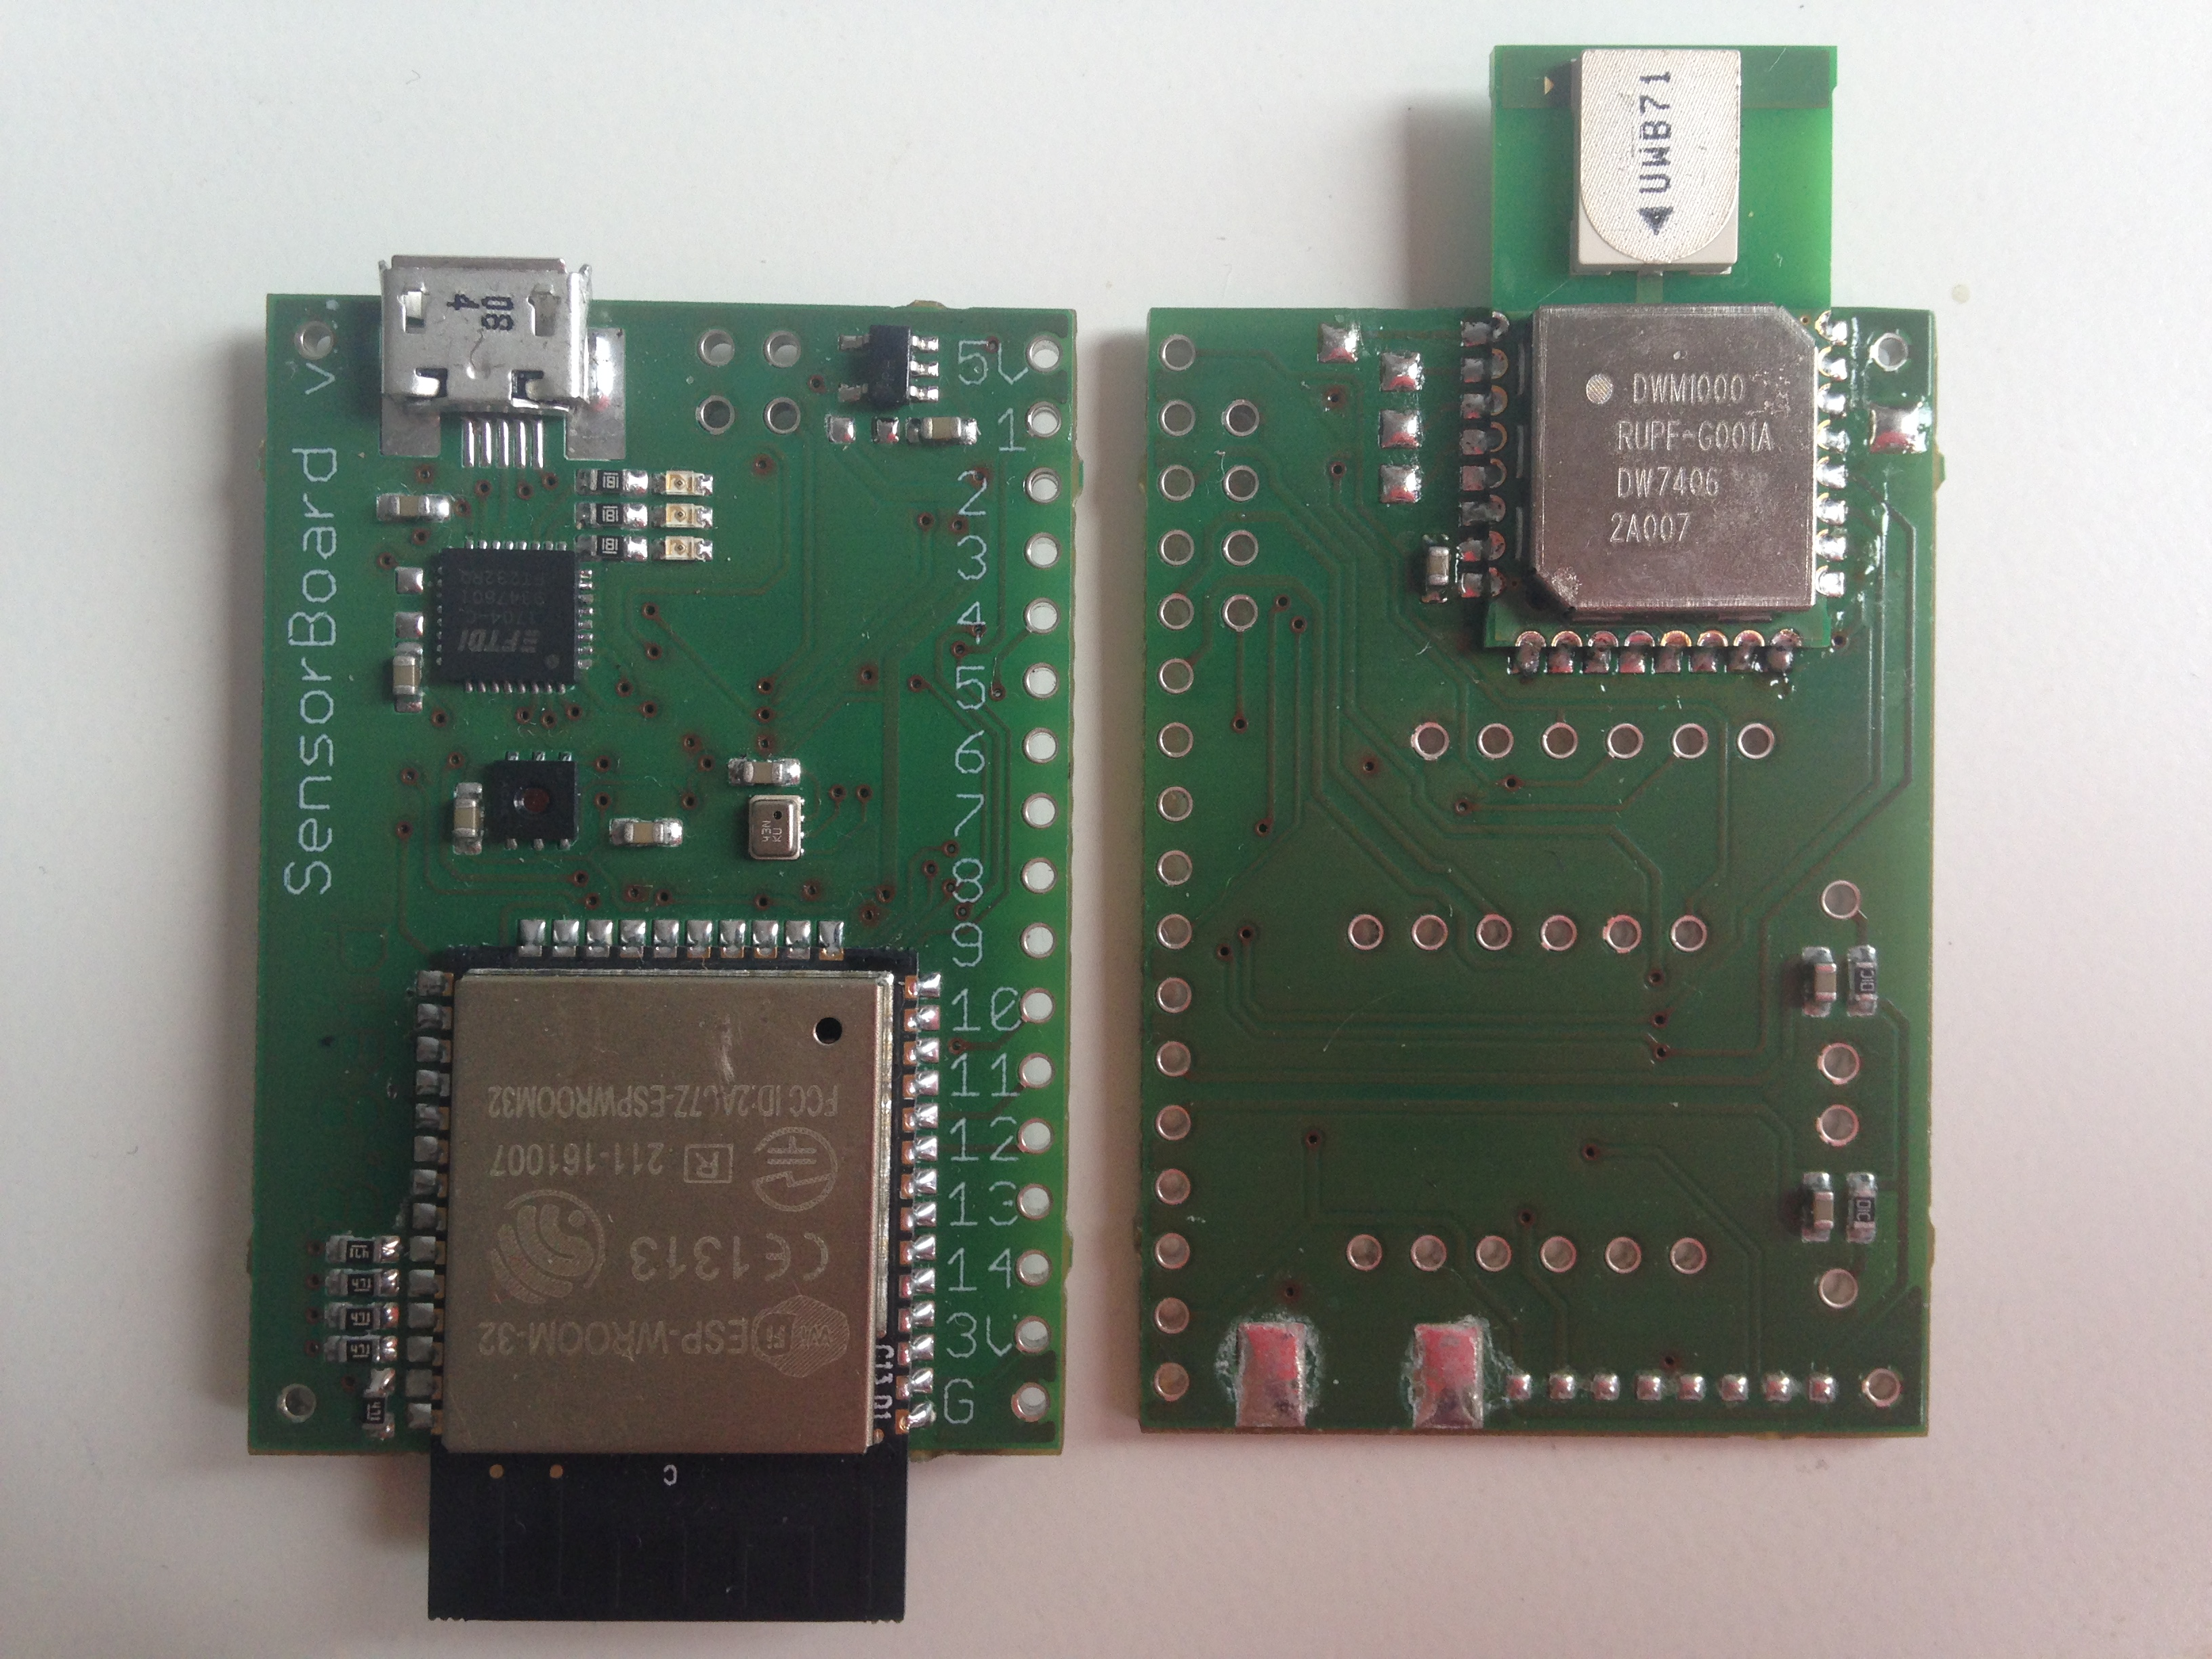
\includegraphics[width=10cm]{img/1.jpg}
    \\\centering Top
  \end{minipage}
  \begin{minipage}{10cm}
    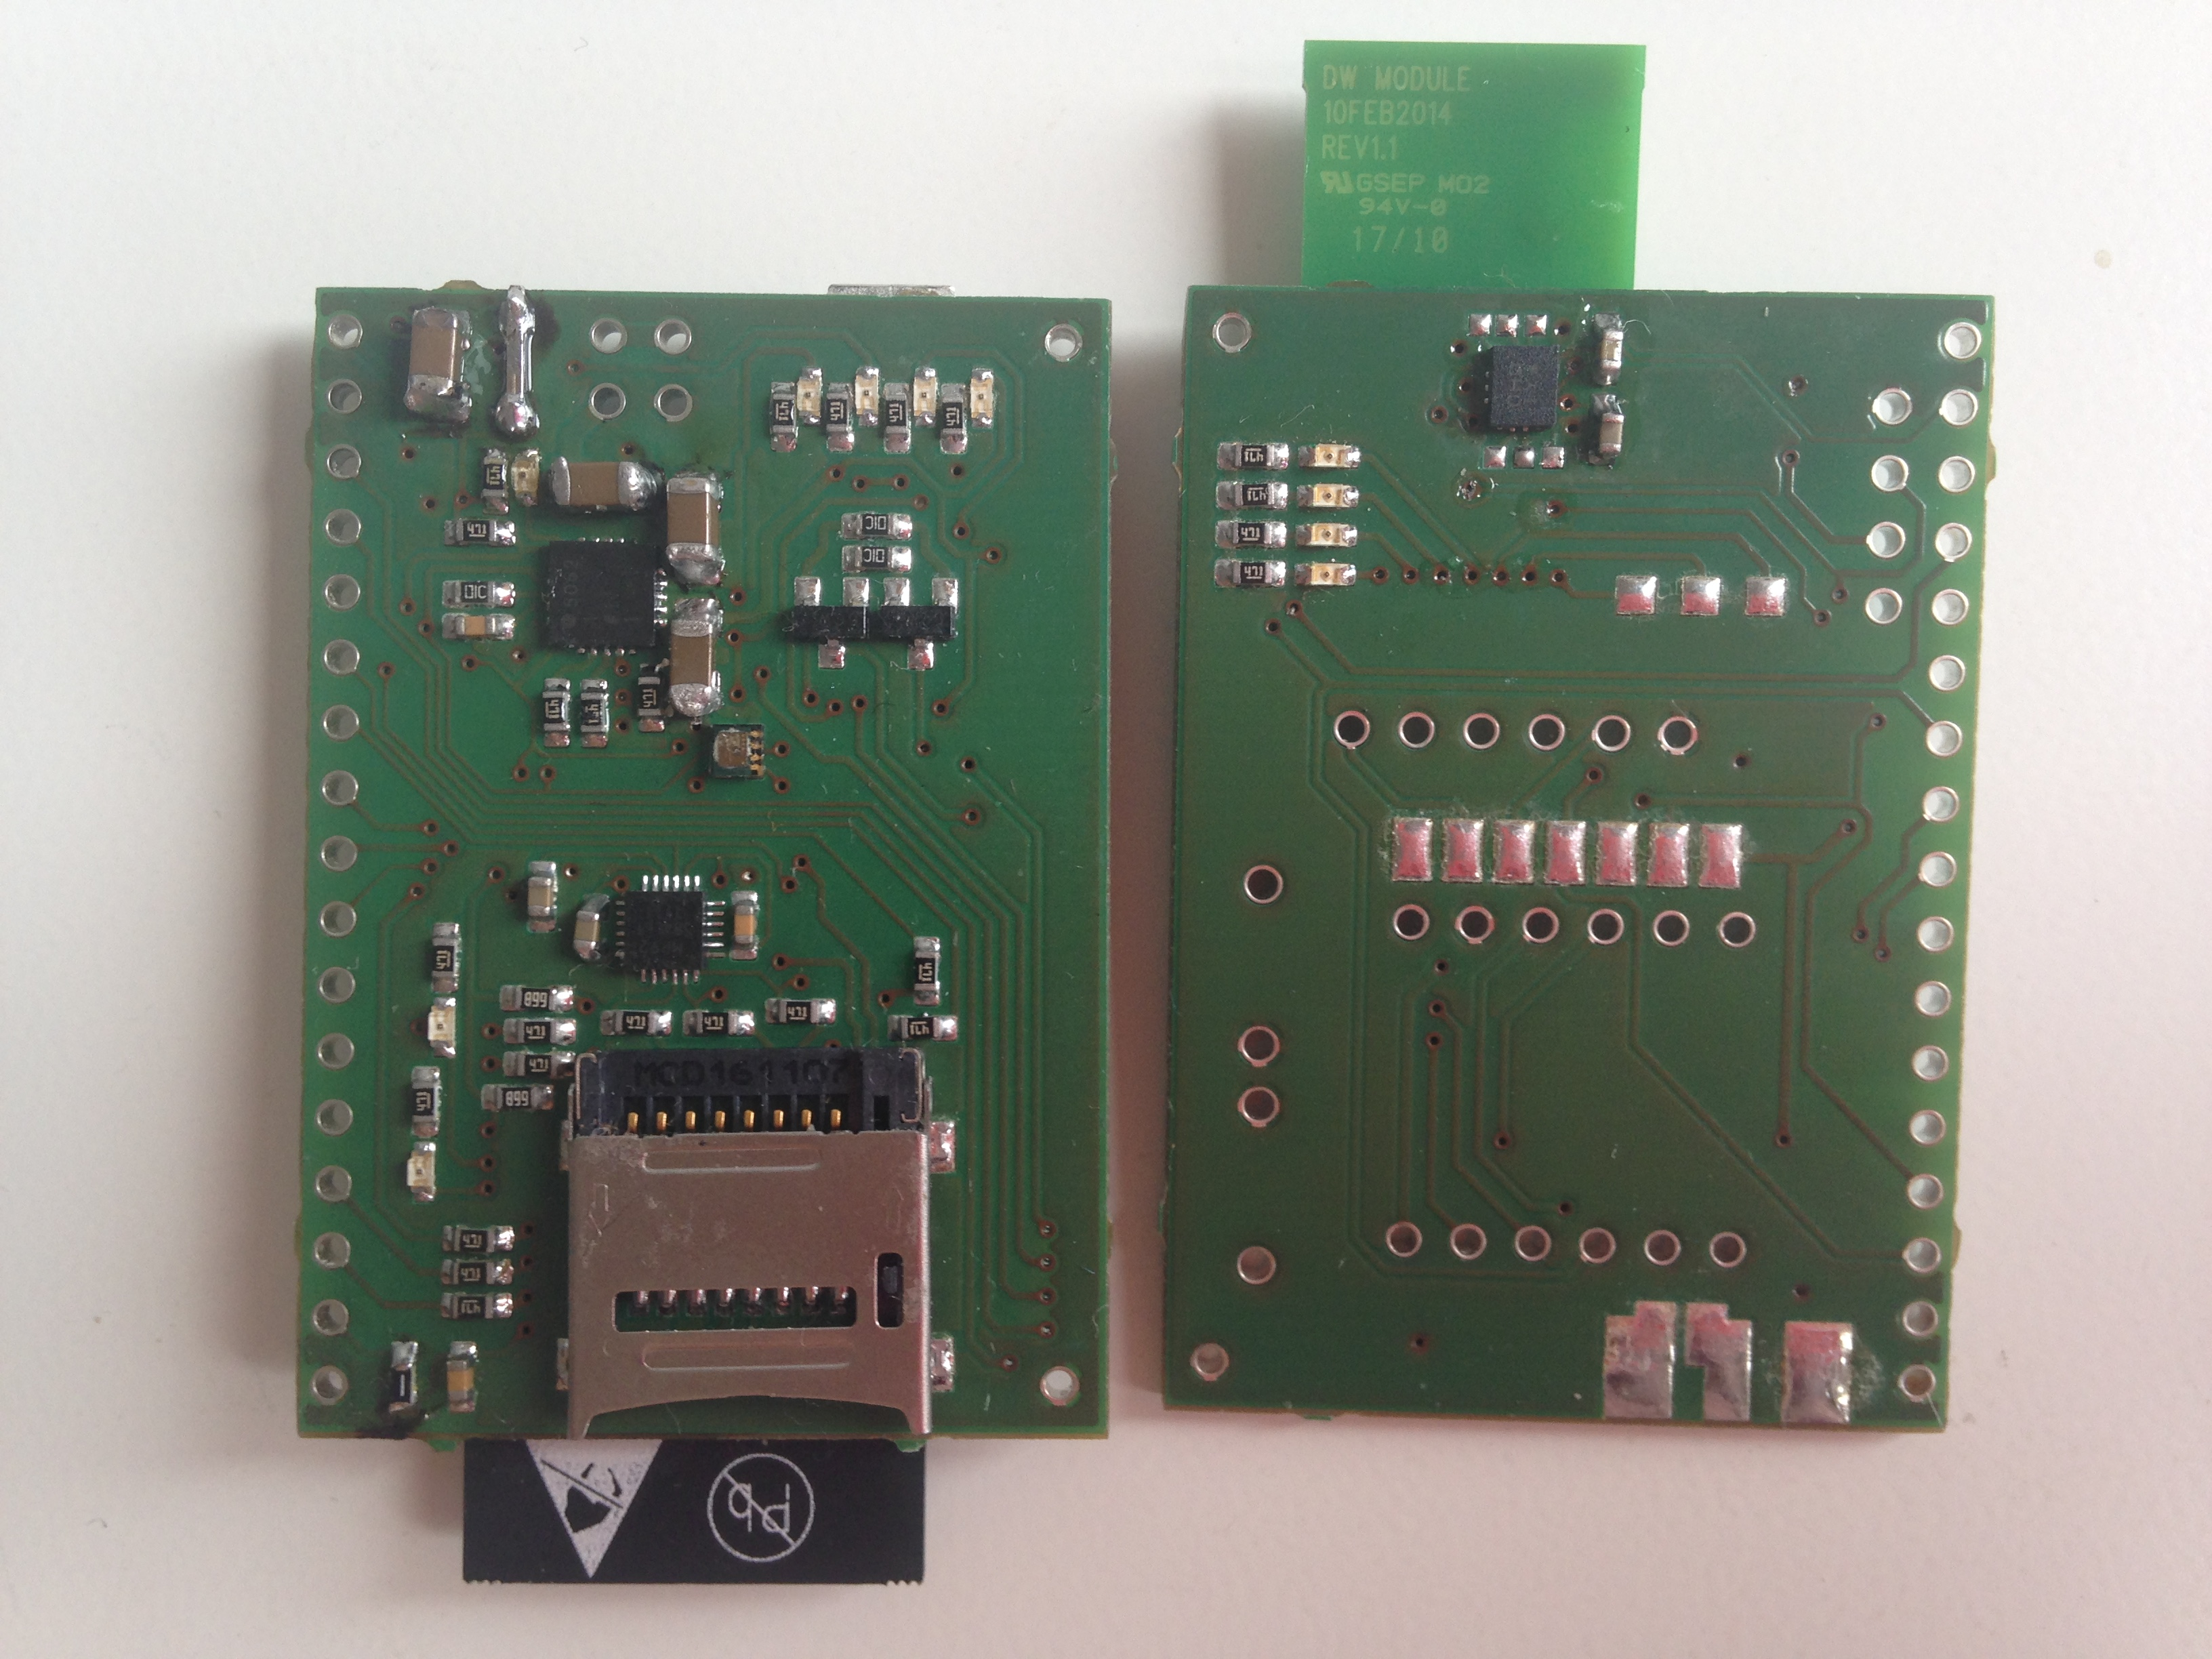
\includegraphics[width=10cm]{img/2.jpg}
    \\\centering Bottom
  \end{minipage}
  \caption{Photo of the prototype boards}
  \label{BoardPhotos}
\end{figure}

\newpage
\tableofcontents

\newpage

\section{HW specifikace SensorBoard}
\begin{itemize}
	\item procesor ESP32 40~MHz
	\item výpočetní koprocesor Atmel ARM 32 bit Cortex M0+
	\item akcelerometr, dynamický gyroskop, kompas, kompatibilní s MetaWear
	\item AHRS senzory integrované v jednom čipu s výpočetním procesorem pro zvýšení přesnosti a zmenšení objemu
	\item logování 100~Hz, $\pm$16~g, $\pm$2000~$^{\circ}/s$
	\item dva nezávislé ACC/GYRO/MAG pro porovnání
	\item teploměr, vlhkoměr, světlocitlivý senzor
	\item DecaWave výpočet relativní polohy $\pm$10 cm
	\item komunikace WiFi, Bluetooth, 433~Mhz radio, 868~MHz radio
	\item komunikace přes USB
	\item přímá konektivita do cloudu nebo přes mobilní telefon
	\item mikro SD karta
	\item mikro USB s možností USB-C
	\item napájení LiPoly, nabíjení přes USB, doba nabíjení cca 1.5~h, výdrž cca 20~h, nastavitelné podle zvolené baterie
	\item obvod pro sledování stavu baterie, ochranu a nabíjení
	\item indikace stavu baterie
	\item programovatelné uživatelem, nový program se nahrává přes USB nebo přes Bluetooth
	\item sensor fusion v reálném čase
	\item při výpadku komunikace se neztratí měřená data, odešlou se hned při obnovení spojení
	\item pokud je k dispozici WiFi síť, data mohou být uploadována přímo na server bez nutnosti používat mobilní telefon
	\item porty na GPS, analogové senzory (mikrofon, srdeční tep, \dots)
	\item výstup 3.3~V a 5~V
	\item možnost zapojení senzorů do jedné sítě, více desek potom ukládá a posílá data jako jeden senzor
	\item synchronní start všech senzorů v síti, možnost synchronizace s kamerou (kamera telefonu nebo kamera se vstupem pro klapku)
	\item dvě tlačítka pro ovládání bez telefonu nebo notebooku
	\item několik indikačních LED
	\item servo kontrolér
\end{itemize}


\section{SW specifikace SensorBoard}

Softwarová specifikace zahrnuje popis algoritmu pro rozpoznávání typu pohybu a funkcionalitu firmwaru měřicího hardwaru. Algoritmus pro rozpoznávání typu pohybu je oddělitelnou součástí firmwaru. Může běžet v reálném čase přímo na měřicícm zařízení nebo například na serveru, na který jsou nahrávána surová naměřená data.

Pro správnou analýzu naměřených dat algoritmus očekává na svém vstupu hodnoty, které:
\begin{itemize}
	\item jsou měřené na konstantní frekvenci, výchozí nastavení je 100 Hz
	\item data ze všech akcelerometrů a gyroskopů jsou pořízena v jeden okamžik
	\item v datech se nenachází saturované úseky (data nedosahují maximální naměřitelné hodnoty)
\end{itemize}


\paragraph{Ukázka uživatelského kódu volaného ve smyčce například ve funkci main:} \quad\\
\Cpp
\begin{lstlisting}
const int frequency = 100; // Hz
HorseAnalysis horse(frequency);

// Load data from sensors to AccX, AccY, AccZ, GyrX, GyrY, GyrZ
horse.addData(AccX, AccY, AccZ, GyrX, GyrY, GyrZ);

// get elapsed time in milliseconds
int elapsedTime = horse.elapsedTime();
// true if horse is moving
bool isMoving = horse.isMoving();
// get number of hoof contacts with ground
int numberOfSteps = horse.numSteps();
// get type of movement as int representing enum
int movementType = horse.detectAndNameMovement();
\end{lstlisting}

\subsection{Způsob práce s daty}
Data jsou algoritmem zpracovávána ihned po svém příchodu. Algoritmus tedy může běžet v reálném čase přímo na zařízení. Algoritmus si ukládá historii několika posledních měření (výchozí nastavení je posledních 5 sekund). Analýza je prováděna postupně v několika vrstvách. V první vrstvě je automaticky nakalibrován vertikální směr a je tak rozlišeno mezi vertikálními a horizontálními pohyby. Ve druhé vrstvě jsou označeny všechny peaky a body zajímavé z hlediska vyšetření průběhu funkce. V dalších vrstvách jsou postupně odhalovány složitější struktury v naměřených datech. K tomu je využívána i ukládaná historie posledních naměřených hodnot. Zároveň jsou z historie počítány statistiky posledních hodnot, které slouží jako jedna ze vstupních informací pro hledání složitejších struktur v datech.

\paragraph{Funkce addData, která volá všechny funkce analyzující data:} \quad\\
\Cpp
\begin{lstlisting}
void addData(double ax, double ay, double az, double gx, double gy, double gz)
{
   updateTime();
   
   updateLastData(
      Vector3D(ax, ay, az),
      Vector3D(gx, gy, gz),
      m_actualMovement
   );
   
   updateZeroOffsets();
   
   updateStatistics();
   
   if(isZeroAcc())
       m_lastZeroTime = m_time;
       
   detectStep();
   
   m_actualMovement = detectMovement();
}
\end{lstlisting}

\subsection{Detekce složitějších struktur v datech}
Společně s označením všech peaků jsou označeny i všechny průchody nulou. Průchod nulou je takový stav akcelerometru, kdy nedochází k žádnému zrychlení a vektorový součet jednotlivých os dává přesně vektor gravitačního zrychlení. Průchod nulou je takový stav gyroskopu, kdy nedochází k žádné změně rychlosti rotace a všechny osy měří nulu. Částečný průchod nulou je takový stav akcelerometru, kdy nedochází k žádnému zrychlení ve vertikální ose, ale může docházet ke zrychlení v horizontální ose. Na základě těchto dat je časová osa rozdělena na úseky, kde každý úsek představuje právě jedno zhoupnutí. Zhoupnutí začíná a končí lokálním bodem s nejnižší hodnotou absolutní akcelerace. Nejnižší hodnota absolutní akcelerace může být až stav bez tíže, což znamená, že se senzor pohybuje volným pádem. Uvnitř každého zhoupnutí se nesmí nacházet nižší hodnota akcelerace než na jeho libovolném okraji.

Jedno zhoupnutí může reprezentovat žádný, jeden, nebo několik dopadů kopyta na zem. Žádný dopad kopyta je detekován v případě, že pohyb koně je vyhodnocen jako stání. V takovém případě se jako zhoupnutí projevuje například dýchání nebo pohyb hlavou. Pokud je detekován pohyb koně, je každý kladný peak vyhodnocen jako dopad kopyta. Na základě statistiky posledních dat jsou odmazány nereálné dopady kopyt. Jedná se o dopady, mezi kterými je naměřen abnormální časový interval nebo mají abnornální amplitudu.

Na základě detekovaných zhoupnutí a dopadů kopyt je vyhodnocován způsob pohybu. Rozlišuje se mezi stáním, krokem, klusem a cvalem. Každý typ pohybu je vyhodnocován na základě jeho definice v daném tvaru. Do zdrojového kódu algoritmu lze snadno vložit defici dalšího pohybu a detekovat jej. Definice každého typu pohybu se skládá ze souboru událostí a každá událost má přiřazenu pravděpodobnost. Jde o pravděpodobnost, že se jedná o daný typ pohybu, pokud tato událost nastala. Algoritmus vyhodnotí všechny události, které nastaly, a vybere pohyb, který je pro tento soubor událostí nejpravděpodobnější. Událost je detekování nějaké struktury v naměřených datech v daný čas. Příklad události je: V poslední sekundě dopadla alespoň tři kopyta s amplitudou alespoň 2G. Všechny události je možné vyhodnotit jako booleovský výraz.

Kvalita definic pro dané typy pohybu je hlavním měřítkem úspěšnosti celé analýzy pohybu. V algoritmu je předpokládáno, že definice budou často upravovány. V případě, že je vyhodnoceno více pohybů se stejnou pravděpodobností, tak je postupováno následovně. Pokud je jedním z pohybů poslední vypočtený pohyb, je zvolen tento poslední vypočtený pohyb. V opačném případě je zvolen pohyb, jehož index je blíže k poslednímu pohybu. Indexy pohybu jsou nyní přířazeny takto: 0 - stání, 1 - krok, 2 - klus, 3 - cval.

\paragraph{Funkce detectMovement, která analyzuje výše zmíněné definice:} \quad\\
\Cpp
\begin{lstlisting}
int detectMovement()
{
	if(!isMoving())
		return 0;

	// (...)
	
	// First definition
	// -------------------- event ---------------------------
	// if the amplitude of last step is more than 5.0 G,
	// -------------------- action --------------------------
	// increase the probability of gallop (cval = 3)
	if(m_lastStep.amplitude > 5.0 /*G*/)
		prob[3]++;
	
	// Second definition
	// -------------------- event ---------------------------
	// if the time from last step is more than 400 ms,
	// and the amplitude of the last step was less than 2.0 G
	// -------------------- action --------------------------
	// increase the probability of walk (krok = 1)
	if(
		m_time - m_lastStep.time > 400 /*ms*/ &&
		m_lastStep.amplitude < 2.0 /*G*/
	)
		prob[1]++;
	
	// other definitions
	// (...)

	return getIndexOfMaxValue(prob, 5 /*size of array prob*/);
}
\end{lstlisting}

\subsection{Kombinace senzorů}
V angličtině se s touto funkcí můžeme setkat pod názvem "Sensor Fusion". Jde o matematickou funkci, která na svém vstupu obdrží naměřená data z více senzorů a na svém výstupu emuluje data naměřená novým senzorem, který se v hardwaru fyzicky nevyskytuje. V našem případě se s touto funkcí setkáme například při emulaci statického gyroskopu (hodnoty pitch, roll a yaw) pomocí dat naměřených akcelerometrem, dynamickým gyroskopem a kompasem. Hodnoty získané touto emulací můžeme použít na algoritmu pro rozpoznání typu pohybu stejně jako hodnoty naměřené fyzickými senzory. Stejně tak můžeme vytvářet definice pohybů, které pracují s emulovanými daty. Pokud některý ze senzorů z nějakého důvodu není k dispozici (včetně emulovaných), jsou všechny definice používající tento senzor ignorovány.

\paragraph{Příklad využití Sensor Fusion v kombinaci akcelerometru, gyroskopu a kompasu pro emulování senzoru absolutní rotace (statického gyroskopu):} \quad\\
\Cpp
\begin{lstlisting}
// output quaternion of sensor frame relative to auxiliary frame
float q0, q1, q2, q3;

MadgwickAHRSupdate(
	float gx, float gy, float gz,  // gyro
	float ax, float ay, float az,  // acc
	float mx, float my, float mz   // mag
);

// q0, q1, q2, q3 ... we have an absolute rotation quaternion
// computed by Madgwick sensor fusion algorithm
\end{lstlisting}

\subsection{Doplňující senzory}
Software je navržen tak, aby bylo možné jednoduše přidat nový senzor a pracovat s jeho hodnotami. V první verzi hardwaru jsou připraveny tyto rozšiřující senzory za účelem jejich otestování:
\begin{itemize}
	\item \textbf{DWM1000:} Senzor relativní polohy v okruhu 300 m s přesností měření 10 cm.
	\item \textbf{GPS:} GPS s výstupem NMEA 2000 na UART 3.3 V
	\item \textbf{Srdeční rytmus:} Senzor srdečního rytmu s analogovým výstupem.
	\item \textbf{Mikrofon:} Mikrofon zapojíme jako analogový senzor a naměřené zvuky nám na určitých částech těla mohou pomoct například v rozpoznání dechu nebo dopadů kopyt.
	\item \textbf{Port pro analogové senzory:} K měřicímu hardwaru můžeme připojit libovolný senzor s analogovým výstupem v rozsahu od 0V po napájecí napětí.
\end{itemize}

\subsection{Konektivita}
Naměřená a případě zpracovaná data mohou být získávána několika způsoby. Asi nejčastěji využívaná metoda je odesílání dat ze senzoru do mobilního telefonu pomocí technologie Bluetooth a následné ukládání v mobilním telefonu nebo odesílání na server. Další možností je ukládat data na mikro SD kartu a následně je odeslat přes USB, Bluetooth nebo WiFi do počítače. Poslední realizovanou technologií je odesílání dat přes UART do vysílajícího modulu s větším dosahem.

Bezdrátová konektivita umožňuje vzájemnou komunikaci mezi více senzory, které jsou použité v rámci jednoho měření. Celá síť se potom chová jako jeden senzor, to znamená, že je možné celou síť připojit například k mobilnímu telefonu jako jeden senzor a naměřená data v reálném čase odesílat na server. V případě, že z jakéhokoliv důvodu dojde k přerušení bezdrátového datového spoje, data jsou automaticky ukládána na mikro SD kartu a po opětovném navázání spojení se zpožděním odeslána. V případě zapojení více senzorů do sítě si opět můžeme vybrat, jestli chceme naměřená data zpracovávat přímo v čipu (pokud to výkon procesoru dovolí), nebo odesílat surová data ke zpracování na server.

\end{document}
